



\tikzset{every picture/.style={line width=0.75pt}} %set default line width to 0.75pt        

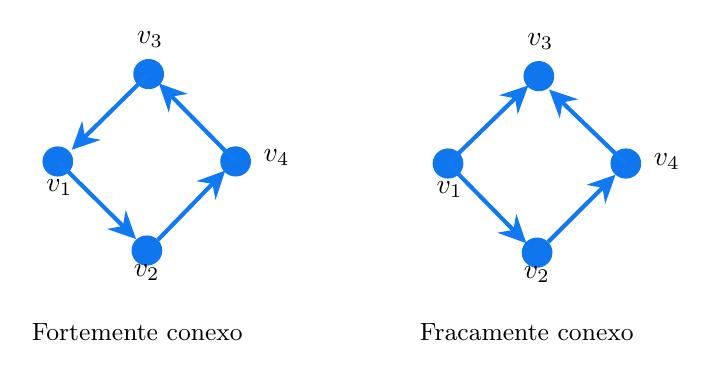
\begin{tikzpicture}[x=0.75pt,y=0.75pt,yscale=-1,xscale=1]
%uncomment if require: \path (0,175); %set diagram left start at 0, and has height of 175

%Shape: Ellipse [id:dp32304183691425004] 
\draw  [draw opacity=0][fill={rgb, 255:red, 15; green, 118; blue, 237 }  ,fill opacity=1 ] (13.01,68.75) .. controls (13.01,64.74) and (16.33,61.48) .. (20.42,61.48) .. controls (24.51,61.48) and (27.83,64.74) .. (27.83,68.75) .. controls (27.83,72.77) and (24.51,76.02) .. (20.42,76.02) .. controls (16.33,76.02) and (13.01,72.77) .. (13.01,68.75) -- cycle ;
%Shape: Ellipse [id:dp8106067468250495] 
\draw  [draw opacity=0][fill={rgb, 255:red, 15; green, 118; blue, 237 }  ,fill opacity=1 ] (55.92,111.67) .. controls (55.92,107.66) and (59.24,104.41) .. (63.33,104.41) .. controls (67.42,104.41) and (70.74,107.66) .. (70.74,111.67) .. controls (70.74,115.69) and (67.42,118.94) .. (63.33,118.94) .. controls (59.24,118.94) and (55.92,115.69) .. (55.92,111.67) -- cycle ;
%Shape: Ellipse [id:dp23696692362251226] 
\draw  [draw opacity=0][fill={rgb, 255:red, 15; green, 118; blue, 237 }  ,fill opacity=1 ] (56.76,26.66) .. controls (56.76,22.64) and (60.08,19.39) .. (64.17,19.39) .. controls (68.26,19.39) and (71.58,22.64) .. (71.58,26.66) .. controls (71.58,30.67) and (68.26,33.93) .. (64.17,33.93) .. controls (60.08,33.93) and (56.76,30.67) .. (56.76,26.66) -- cycle ;
%Shape: Ellipse [id:dp8830615362278031] 
\draw  [draw opacity=0][fill={rgb, 255:red, 15; green, 118; blue, 237 }  ,fill opacity=1 ] (98.67,68.75) .. controls (98.67,64.74) and (101.99,61.48) .. (106.08,61.48) .. controls (110.17,61.48) and (113.49,64.74) .. (113.49,68.75) .. controls (113.49,72.77) and (110.17,76.02) .. (106.08,76.02) .. controls (101.99,76.02) and (98.67,72.77) .. (98.67,68.75) -- cycle ;
%Straight Lines [id:da5307131229877817] 
\draw [color={rgb, 255:red, 16; green, 121; blue, 243 }  ,draw opacity=1 ][fill={rgb, 255:red, 0; green, 0; blue, 0 }  ,fill opacity=1 ][line width=1.5]    (29.96,60.34) -- (64.17,26.66) ;
\draw [shift={(27.11,63.14)}, rotate = 315.45] [fill={rgb, 255:red, 16; green, 121; blue, 243 }  ,fill opacity=1 ][line width=0.08]  [draw opacity=0] (13.4,-6.43) -- (0,0) -- (13.4,6.44) -- (8.9,0) -- cycle    ;
%Straight Lines [id:da7377027091982162] 
\draw [color={rgb, 255:red, 16; green, 121; blue, 243 }  ,draw opacity=1 ][fill={rgb, 255:red, 0; green, 0; blue, 0 }  ,fill opacity=1 ][line width=1.5]    (106.08,68.75) -- (71.91,33.99) ;
\draw [shift={(69.11,31.14)}, rotate = 405.5] [fill={rgb, 255:red, 16; green, 121; blue, 243 }  ,fill opacity=1 ][line width=0.08]  [draw opacity=0] (13.4,-6.43) -- (0,0) -- (13.4,6.44) -- (8.9,0) -- cycle    ;
%Straight Lines [id:da03378894348995787] 
\draw [color={rgb, 255:red, 16; green, 121; blue, 243 }  ,draw opacity=1 ][fill={rgb, 255:red, 0; green, 0; blue, 0 }  ,fill opacity=1 ][line width=1.5]    (20.42,68.75) -- (55.27,103.32) ;
\draw [shift={(58.11,106.14)}, rotate = 224.77] [fill={rgb, 255:red, 16; green, 121; blue, 243 }  ,fill opacity=1 ][line width=0.08]  [draw opacity=0] (13.4,-6.43) -- (0,0) -- (13.4,6.44) -- (8.9,0) -- cycle    ;
%Straight Lines [id:da7335741593118423] 
\draw [color={rgb, 255:red, 16; green, 121; blue, 243 }  ,draw opacity=1 ][fill={rgb, 255:red, 0; green, 0; blue, 0 }  ,fill opacity=1 ][line width=1.5]    (68.63,106.56) -- (98.32,76.01) ;
\draw [shift={(101.11,73.14)}, rotate = 494.19] [fill={rgb, 255:red, 16; green, 121; blue, 243 }  ,fill opacity=1 ][line width=0.08]  [draw opacity=0] (13.4,-6.43) -- (0,0) -- (13.4,6.44) -- (8.9,0) -- cycle    ;
%Shape: Ellipse [id:dp7206263546182852] 
\draw  [draw opacity=0][fill={rgb, 255:red, 15; green, 118; blue, 237 }  ,fill opacity=1 ] (201.01,69.75) .. controls (201.01,65.74) and (204.33,62.48) .. (208.42,62.48) .. controls (212.51,62.48) and (215.83,65.74) .. (215.83,69.75) .. controls (215.83,73.77) and (212.51,77.02) .. (208.42,77.02) .. controls (204.33,77.02) and (201.01,73.77) .. (201.01,69.75) -- cycle ;
%Shape: Ellipse [id:dp4735230927400256] 
\draw  [draw opacity=0][fill={rgb, 255:red, 15; green, 118; blue, 237 }  ,fill opacity=1 ] (243.92,112.67) .. controls (243.92,108.66) and (247.24,105.41) .. (251.33,105.41) .. controls (255.42,105.41) and (258.74,108.66) .. (258.74,112.67) .. controls (258.74,116.69) and (255.42,119.94) .. (251.33,119.94) .. controls (247.24,119.94) and (243.92,116.69) .. (243.92,112.67) -- cycle ;
%Shape: Ellipse [id:dp10240481582403205] 
\draw  [draw opacity=0][fill={rgb, 255:red, 15; green, 118; blue, 237 }  ,fill opacity=1 ] (244.76,27.66) .. controls (244.76,23.64) and (248.08,20.39) .. (252.17,20.39) .. controls (256.26,20.39) and (259.58,23.64) .. (259.58,27.66) .. controls (259.58,31.67) and (256.26,34.93) .. (252.17,34.93) .. controls (248.08,34.93) and (244.76,31.67) .. (244.76,27.66) -- cycle ;
%Shape: Ellipse [id:dp699203588972158] 
\draw  [draw opacity=0][fill={rgb, 255:red, 15; green, 118; blue, 237 }  ,fill opacity=1 ] (286.67,69.75) .. controls (286.67,65.74) and (289.99,62.48) .. (294.08,62.48) .. controls (298.17,62.48) and (301.49,65.74) .. (301.49,69.75) .. controls (301.49,73.77) and (298.17,77.02) .. (294.08,77.02) .. controls (289.99,77.02) and (286.67,73.77) .. (286.67,69.75) -- cycle ;
%Straight Lines [id:da3863788592313979] 
\draw [color={rgb, 255:red, 16; green, 121; blue, 243 }  ,draw opacity=1 ][fill={rgb, 255:red, 0; green, 0; blue, 0 }  ,fill opacity=1 ][line width=1.5]    (208.42,69.75) -- (244.24,34.93) ;
\draw [shift={(247.11,32.14)}, rotate = 495.81] [fill={rgb, 255:red, 16; green, 121; blue, 243 }  ,fill opacity=1 ][line width=0.08]  [draw opacity=0] (13.4,-6.43) -- (0,0) -- (13.4,6.44) -- (8.9,0) -- cycle    ;
%Straight Lines [id:da3796347012856618] 
\draw [color={rgb, 255:red, 16; green, 121; blue, 243 }  ,draw opacity=1 ][fill={rgb, 255:red, 0; green, 0; blue, 0 }  ,fill opacity=1 ][line width=1.5]    (294.08,69.75) -- (259.99,36.92) ;
\draw [shift={(257.11,34.14)}, rotate = 403.93] [fill={rgb, 255:red, 16; green, 121; blue, 243 }  ,fill opacity=1 ][line width=0.08]  [draw opacity=0] (13.4,-6.43) -- (0,0) -- (13.4,6.44) -- (8.9,0) -- cycle    ;
%Straight Lines [id:da7333948279152087] 
\draw [color={rgb, 255:red, 16; green, 121; blue, 243 }  ,draw opacity=1 ][fill={rgb, 255:red, 0; green, 0; blue, 0 }  ,fill opacity=1 ][line width=1.5]    (208.42,69.75) -- (243.31,105.29) ;
\draw [shift={(246.11,108.14)}, rotate = 225.53] [fill={rgb, 255:red, 16; green, 121; blue, 243 }  ,fill opacity=1 ][line width=0.08]  [draw opacity=0] (13.4,-6.43) -- (0,0) -- (13.4,6.44) -- (8.9,0) -- cycle    ;
%Straight Lines [id:da27556784269755696] 
\draw [color={rgb, 255:red, 16; green, 121; blue, 243 }  ,draw opacity=1 ][fill={rgb, 255:red, 0; green, 0; blue, 0 }  ,fill opacity=1 ][line width=1.5]    (256.63,107.56) -- (286.28,77.97) ;
\draw [shift={(289.11,75.14)}, rotate = 495.06] [fill={rgb, 255:red, 16; green, 121; blue, 243 }  ,fill opacity=1 ][line width=0.08]  [draw opacity=0] (13.4,-6.43) -- (0,0) -- (13.4,6.44) -- (8.9,0) -- cycle    ;

% Text Node
\draw (13.43,75.78) node [anchor=north west][inner sep=0.75pt]    {$v_{1}$};
% Text Node
\draw (55.5,117.05) node [anchor=north west][inner sep=0.75pt]    {$v_{2}$};
% Text Node
\draw (57.18,4.8) node [anchor=north west][inner sep=0.75pt]    {$v_{3}$};
% Text Node
\draw (118.09,61.42) node [anchor=north west][inner sep=0.75pt]    {$v_{4}$};
% Text Node
\draw (6.39,145.44) node [anchor=north west][inner sep=0.75pt]  [font=\small] [align=left] {Fortemente conexo};
% Text Node
\draw (201.43,76.78) node [anchor=north west][inner sep=0.75pt]    {$v_{1}$};
% Text Node
\draw (243.5,118.05) node [anchor=north west][inner sep=0.75pt]    {$v_{2}$};
% Text Node
\draw (245.18,5.8) node [anchor=north west][inner sep=0.75pt]    {$v_{3}$};
% Text Node
\draw (306.09,63.42) node [anchor=north west][inner sep=0.75pt]    {$v_{4}$};
% Text Node
\draw (193.39,145.44) node [anchor=north west][inner sep=0.75pt]  [font=\small] [align=left] {Fracamente conexo};


\end{tikzpicture}